Els plàstics centellejadors son plàstics dopats amb molècules fluorescents, els quals són utilitzats per detectar les partícules de interès. Aquests es poden mecanitzar de moltes formes diferents, de entre les quals, la utilitzada pel projecte TRITIUM és en forma de fibra amb $1~\mm$ o $2~\mm$ de diàmetre i $20~\cm$ de longitud (detector de triti) i en forma de bloc de $17\times 45~\cm^2$ i un gruix de $1~\cm$. 

En els plàstics centellejadors, les partícules que el travessen depositen part de la seua energia cinètica, la qual excita els electrons de les partícules fluorescents. Finalment aquests electrons es desexciten en qüestió de nanosegons mitjançant un procés anomenat fluorescència, a través del qual emiteixen fotons a una longitud de ona que pertany a l'espectre visible. Aquest espectre d'emisió presenta un pic centrat a una longitud d'ona que depèn de la molècula fluorescent utilitzada. En el cas dels plàstics centellejadors utilitzats en el projecte TRITIUM, la molècula fluorescent utilitzada és el fluor, el cual presenta un pic de emissió al voltant dels $435~\nano\meter$, com es pot comprovar en la Figura \ref{fig:EspectreEmisioPlasticsTRITIUM}.

\begin{figure}
\centering
    \begin{subfigure}[b]{0.7\textwidth}
    \centering
    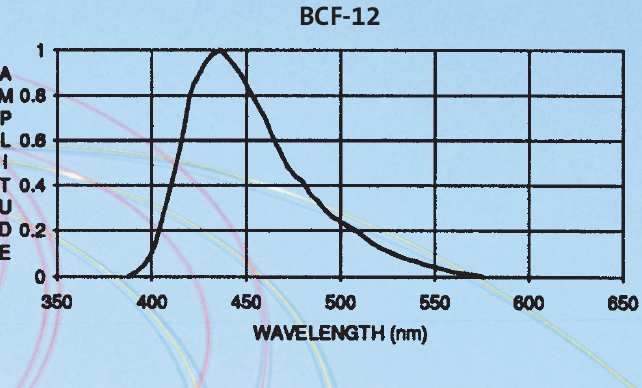
\includegraphics[width=\textwidth]{12Summary/3DesignPrinciples/32Tritium_detector/EmisionBCF12.png}  
        \caption{}\label{subfig:EspectreEmisioFibres}
    \end{subfigure}
    \hfill
    \begin{subfigure}[b]{0.7\textwidth}
    \centering
    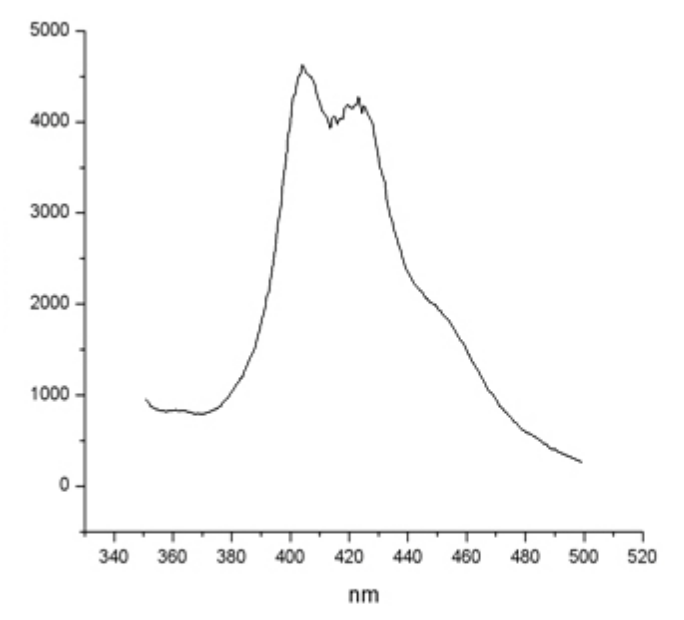
\includegraphics[width=\textwidth]{12Summary/3DesignPrinciples/34BackgroundRejectionSystem/EmissionEnergySpectrumVetos.png}  
    \caption{\label{subfig:EspectreEmisioVeto}}
    \end{subfigure}
\caption{Espectre d'emissió de a) les fibres centellejadores de Saint Gobain, model BCF-12 (utilitzades en el detector de triti) \cite{DataSheetBCF12Fiber} b) bloc de plàstic centellejador d'Epic Crystals (utilitzat en el sistema de rebuig del fons radioactiu)\cite{ScintillatorVeto}\label{fig:EspectreEmisioPlasticsTRITIUM}.}
\end{figure}

Els fotons generats en cada partícula detectada presenten una energia similar però no idèntica ja que el aquests esdeveniments estan descrit per una estadística poissoniana. A més, la quantitat de fotons que es produeixen depèn linealment de la quantitat d'energía depositada dins de un rang d'energies de la partícula.

La col·laboració TRITIUM ha realitzat alguns estudis per quantificar algunes de les propietats més rellevants d'aquestes fibres per al projecte TRITIUM, com ara la dispersió en el nombre de fotons a un mateix esdeveniment o l'eficiència de col·lecció de fotons, obtenint $2.86\%$ i $(76 \pm 8)\%$ respectivament. També s'ha desenvolupat un mètode per incrementar la quantitat de senyal llegida pels fotosensors que consisteix en tallar, polir i netejar les fibres seguint uns protocols adecuats. Per això va caldre desenvolupar diferents màquines, les quals es mostren a la Figura \ref{fig:MaquinesTRITIUM}, basades en tecnologia arduino. També va caldre necessari accedir a l'interior d'una sala blanca per garantir un alt grau de neteja. La millora obtinguda degut a aquest mètode es va quantificar en més de un factor dos. 

\begin{figure}
\centering
    \begin{subfigure}[b]{0.5\textwidth}
    \centering
    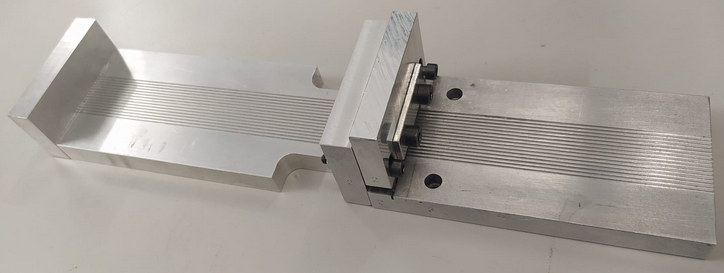
\includegraphics[width=\textwidth]{12Summary/4ResearchAndDevelopments/41Fibers/CuttingDeviceVS.png}  
    \caption{\label{subfig:MaquinaTallar}}
    \end{subfigure}
    \hfill
    \begin{subfigure}[b]{0.45\textwidth}
    \centering
    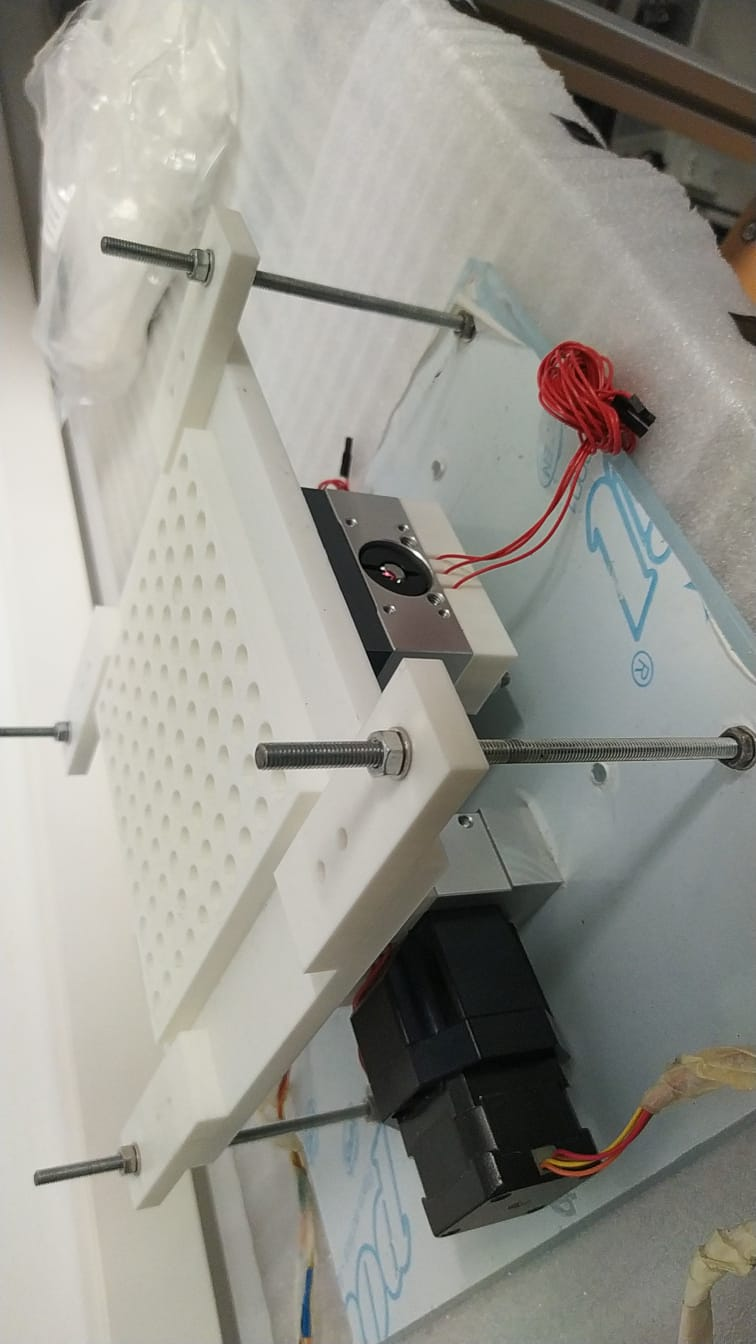
\includegraphics[angle=-90, width=\textwidth]{12Summary/4ResearchAndDevelopments/41Fibers/PolishingTable.jpeg}  
    \caption{\label{subfig:MaquinaPolir}}
    \end{subfigure}
 \caption{Màquines desenvolupades al projecte TRITIUM per a a) tallar fibres centellejadores i b) polir fibres centellejadores en massa. \label{fig:MaquinesTRITIUM}}
\end{figure}